\section{Introduction}
\label{sec:intro}

% Paragraph 1: LLMs are ready: Improved capabilities of LLMs can unlock new applications in scientific research. 
% Automating research is beneficial for society: Scientific research is bottlenecked by human expertise and we want to use research agents to accelerate this process. 
The rapid improvement of LLMs, especially in capabilities like knowledge and reasoning, has enabled many new applications in scientific tasks, such as solving challenging mathematical problems~\cite{Trinh2024SolvingOG}, assisting scientists in writing proofs~\cite{Collins2024EvaluatingLM}, retrieving related works~\cite{Ajith2024LitSearchAR,Press2024CiteMECL}, generating code to solve analytical or computational tasks~\cite{Huang2023MLAgentBenchEL,Tian2024SciCodeAR}, and discovering patterns in large text corpora~\cite{Zhong2023GoalDD,Lam2024ConceptIA}.
% Going further, the capability of LLMs to autonomously perform research and ideation has been central to many discussions on the benefits and risks of future AI systems, and many recent papers have attempted to instantiate systems that act as autonomous research agents~\cite{Wang2023SciMONSI,Baek2024ResearchAgentIR,Yang2023LargeLM,AIScientist,Li2024MLRCopilotAM}.
While these are useful applications that can potentially increase the productivity of researchers, it remains an open question whether LLMs can take on the more creative and challenging parts of the research process.


\begin{figure}[t]
\small
\centering
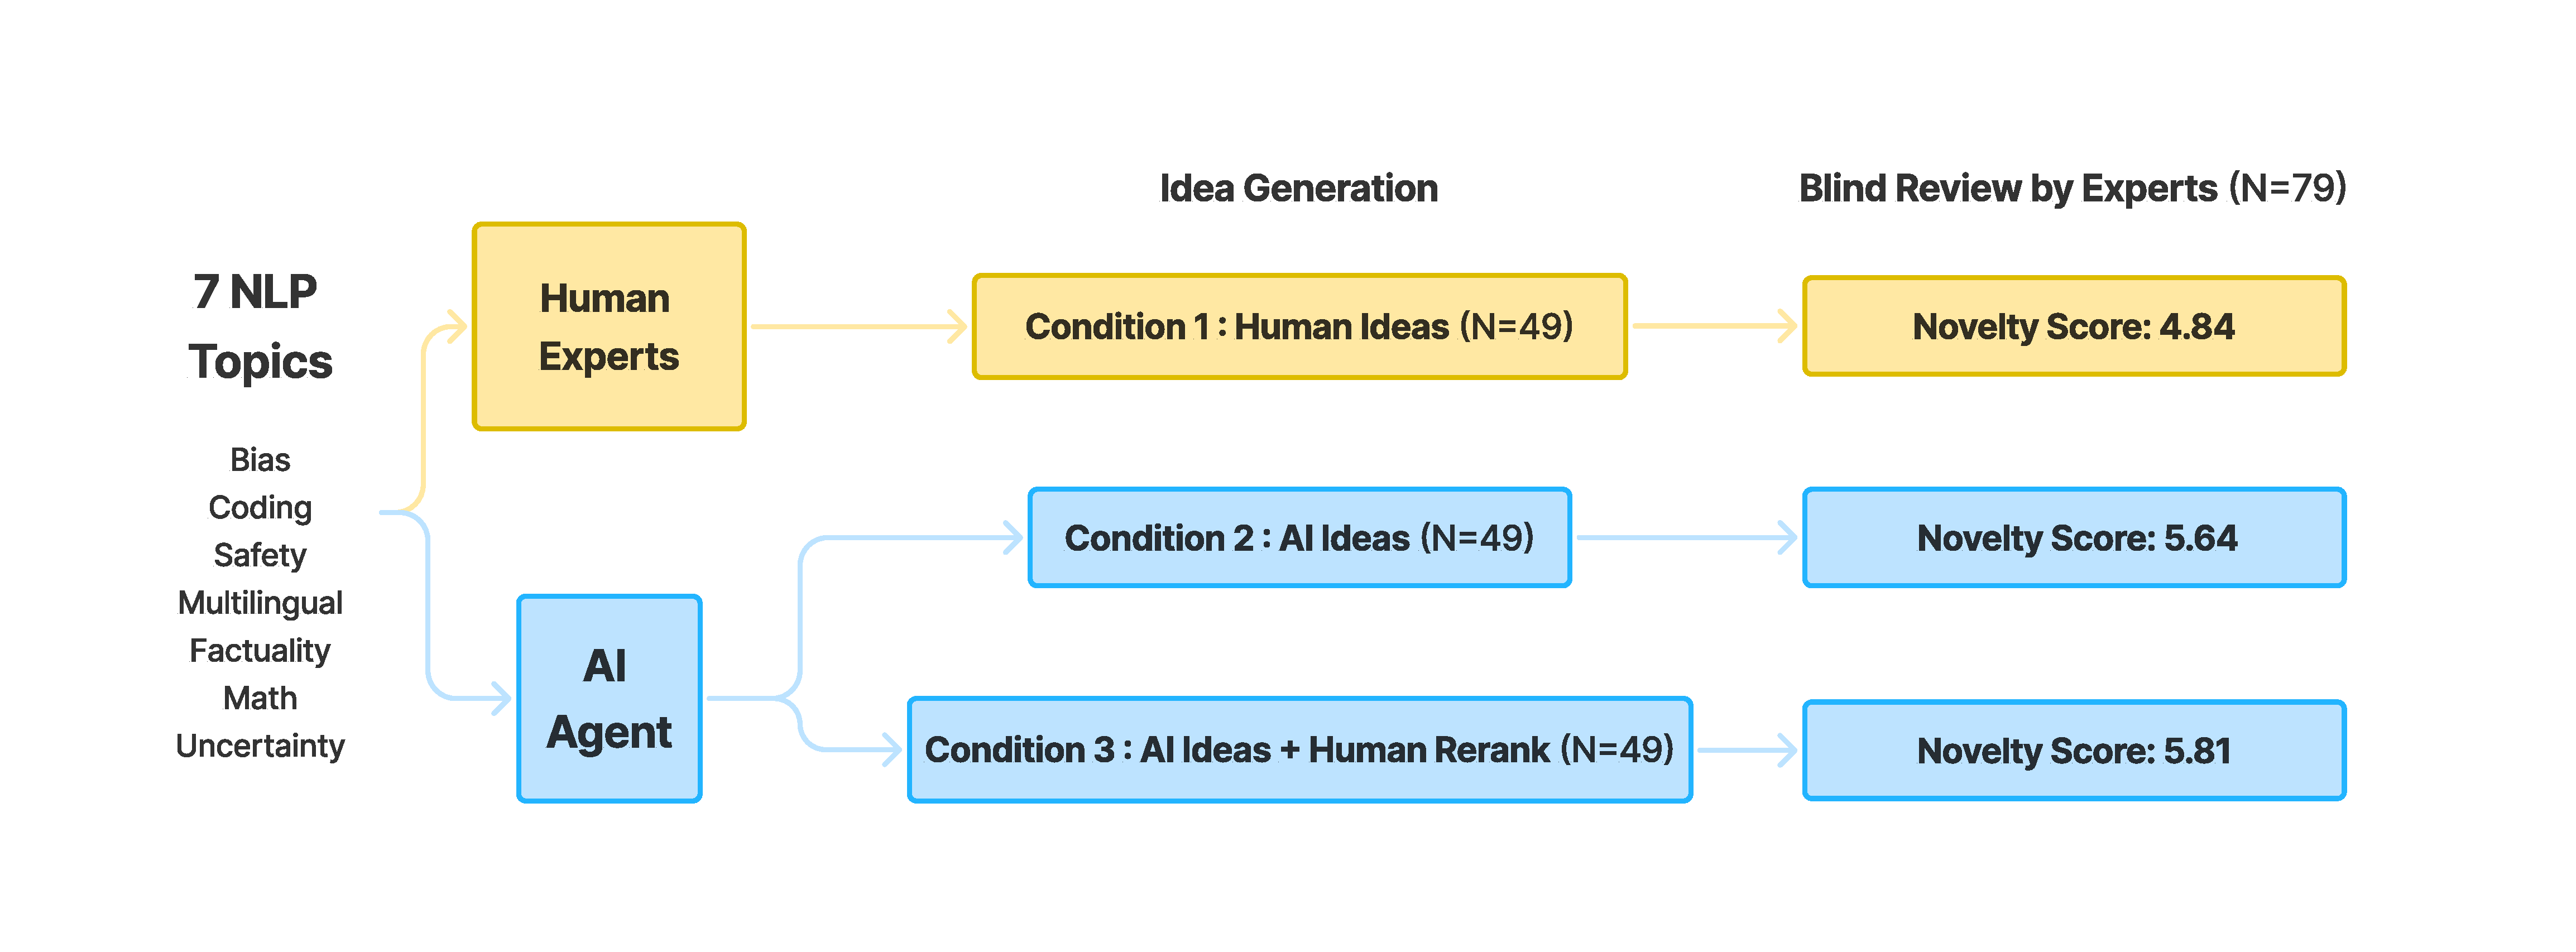
\includegraphics[trim=0 50 0 0,clip,width=\textwidth]{figures/flow_chart.pdf}
\caption{Overview of our study: we recruit 79 expert researchers to perform blind review of 49 ideas from each of the three conditions: expert-written ideas, AI-generated ideas, and AI-generated ideas reranked by a human expert. We standardize the format and style of ideas from all conditions before the blind review. We find AI ideas are judged as significantly more novel than human ideas ($p<0.05$).}
\label{fig:overview}
\end{figure}



% \begin{table}[t]
% \centering
% \small 
% \begin{tabular}{l c c} 
%  \hline
% & Expert Baseline & Expert Evaluation \\ 
% \hline 
% AI Scientist~\cite{AIScientist} & \rxmark & \rxmark \\
% ResearchAgent~\cite{Baek2024ResearchAgentIR} & \rxmark & $N = 10$ \\
% SciMON~\cite{Wang2023SciMONSI} & \rxmark & $N = 6$ \\ 
% MOOSE~\cite{Yang2023LargeLM} & \rxmark & $N =3$ \\
% MLR-Copilot~\cite{Li2024MLRCopilotAM} & \rxmark & $N =3$ \\
% \hline 
% Ours & $N = 49$ & $N = 79$ \\
%  \hline
% \end{tabular}
% \caption{Comparison of evaluation protocols with prior works on research idea generation. We are the first to establish a rigorous human expert baseline and we conducted the largest scale expert evaluation of both expert-written ideas and AI-generated ideas.}
% \label{table:prior_work}
% \end{table}



\begin{figure}[t]
\small
\centering
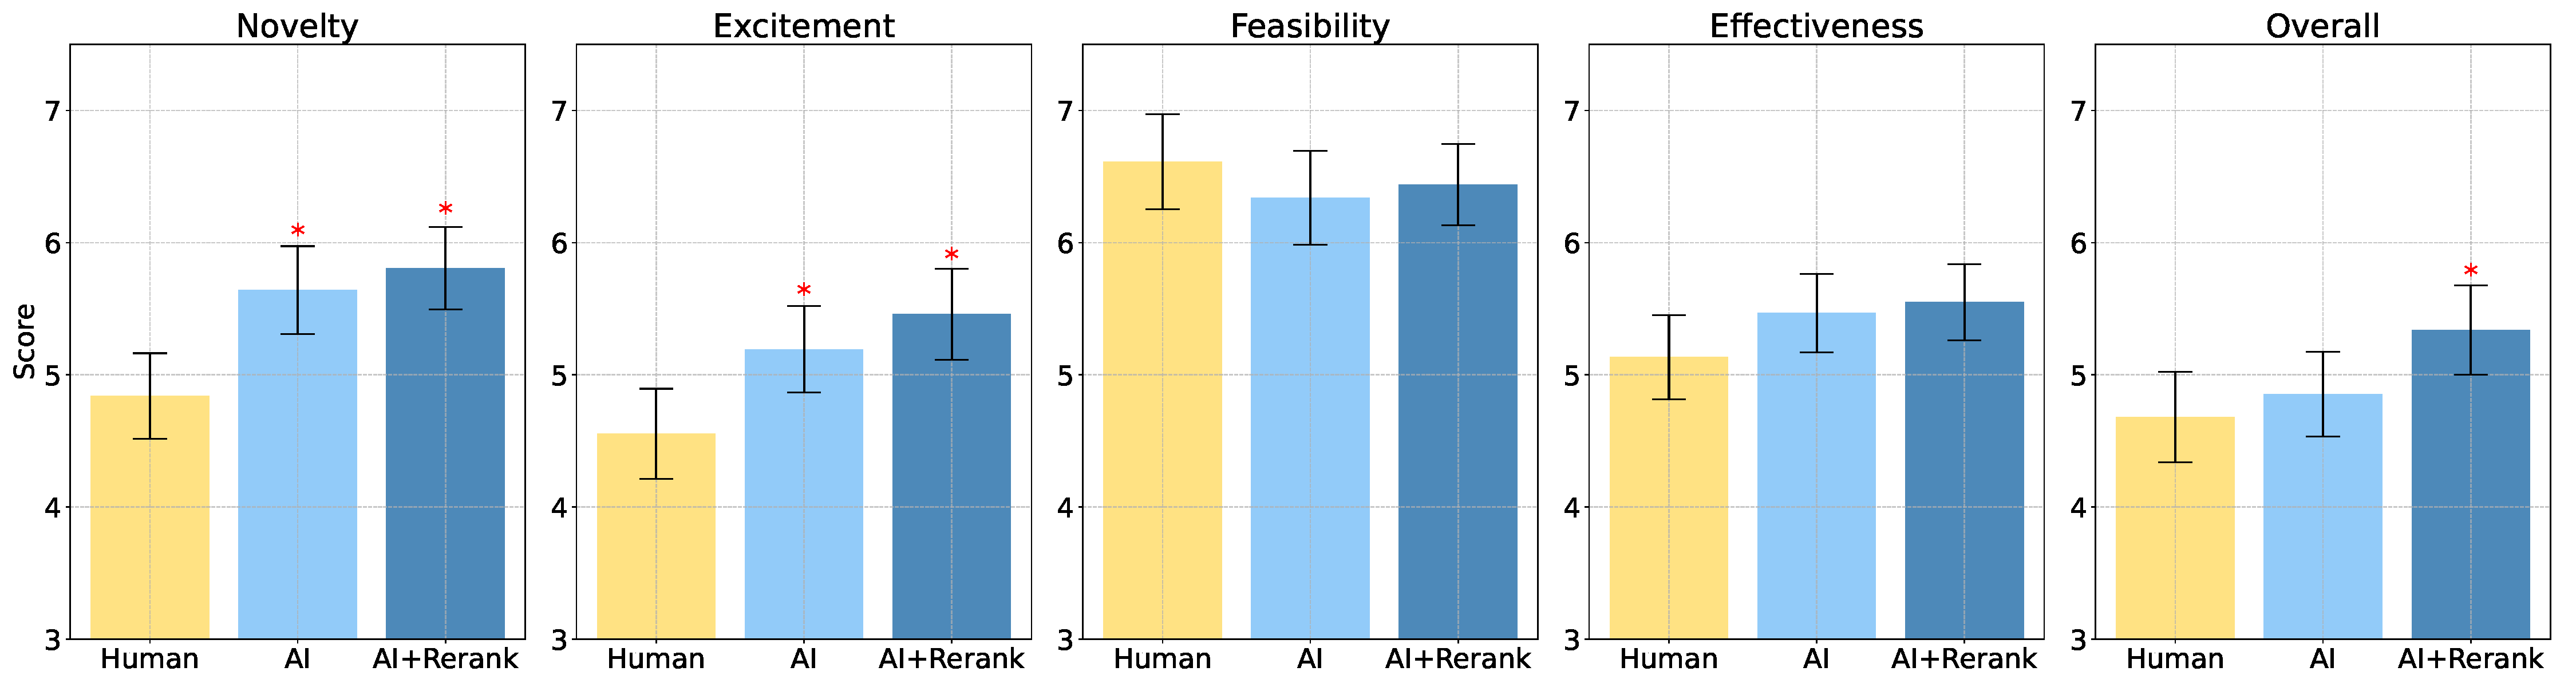
\includegraphics[trim=0 0 0 0,clip,width=\textwidth]{figures/barplots_all_metrics.pdf}
\caption{Comparison of the three experiment conditions across all review metrics. Red asterisks indicate that the condition is statistically better than the \texttt{Human} baseline with two-tailed Welch's t-tests and Bonferroni correction. All scores are on a 1 to 10 scale. More detailed results are in Section~\ref{sec:results}.}
\label{fig:results_barplots}
\end{figure}


We focus on this problem of measuring the  \emph{research ideation} capabilities of LLMs and ask: are current LLMs capable of generating novel ideas that are comparable to expert humans? Although ideation is only one part of the research process, this is a key question to answer, as it is the very first step to the scientific research process and serves as a litmus test for the possibility of autonomous research agents that create their own ideas.
%We study research ideation in particular, which is arguably the most fundamental step of the entire scientific research process.
%
Evaluating expert-level capabilities of LLM systems is challenging~\cite{Bakhtin2022HumanlevelPI,Collins2024EvaluatingLM}, and research ideation takes this to an extreme. Qualified expert researchers are difficult to recruit at scale, evaluation criteria can be highly subjective, and it is difficult for even the best experts to judge the quality of an idea~\cite{beygelzimer2021neurips,Simsek2024DoGP}.


%Despite the prior attempts focused on instantiating research agents, major open problems in evaluation hinder progress. 
%
%First, we do not know whether LLMs are capable of producing novel research ideas, on-par with human experts, which is the foundation for LLMs to produce useful research. 
%Existing works have focused on building agent systems, and their evaluations never compare AI-generated ideas with human experts' ideas, making it difficult to know whether the resulting ideas are comparable at all to experts.
%
% Second, there lacks a well-defined task format for this new problem of research idea generation. Existing works mostly generate short and vague ideas without structured scaffolding and clear executable instructions, limiting their feasibility in downstream execution. 
%
%More recently, LLMs have been envisioned to autonomously perform ideation and even execute the entire research pipeline~\cite{Wang2023SciMONSI,Baek2024ResearchAgentIR,Yang2023LargeLM,AIScientist,Li2024MLRCopilotAM}.
% ,
% leading to discussions on the benefits and risks of future AI systems
%
%Moreover, existing evaluation of AI-generated ideas has generally relied on automatic evaluation by LLMs (which we find to be unreliable in section~\ref{sec:self_eval}), or small-scale human evaluations which lack sufficient statistical power. 
%
%Such evaluations make it impossible to draw statistically meaningful conclusions on LLMs' ideation abilities. 
%These problems are not simple to address, as they require a large-scale evaluation, where expert researchers contribute research ideas  and perform high-quality blind reviews.
%
%This calls for a more rigorous evaluation that would allow us to answer the above question convincingly. 

We address these challenges directly, recognizing that for important, high-stakes tasks like research ideation, there is no substitute for a large-scale expert evaluation. We design a carefully controlled comparison of human and LLM ideas that overcomes sample size and baseline problems present in earlier small-scale evaluation studies. Our study recruited a large pool of over 100 highly qualified NLP researchers to produce human baseline ideas and perform blind reviews of human and LLM ideas. To reduce the possibility that confounding variables affect our outcome measures, we enforce strict controls that standardize the styles of human and LLM ideas and match their topic distribution.

We compare our human expert baseline with a simple and effective LLM agent that incorporates retrieval augmentation and adopts recent ideas in inference-time scaling, such as overgenerating and reranking LM outputs. 
These measures allow us to make statistically rigorous comparisons between human experts and state-of-the-art LLMs (Figure~\ref{fig:overview}). 

Our evaluation-centric approach complements many recent methods-centric works that attempt to instantiate research agents~\cite{Wang2023SciMONSI,Baek2024ResearchAgentIR,Yang2023LargeLM,AIScientist,Li2024MLRCopilotAM}. 
The majority of these works rely on fast and lower-cost evaluation surrogates -- either by decreasing the number of expert reviewers~\cite{Baek2024ResearchAgentIR,Li2024MLRCopilotAM,Wang2023SciMONSI,Yang2023LargeLM}, constraining the length and detailedness of the ideas~\cite{Wang2023SciMONSI,Yang2023LargeLM}, or relying on LLM-as-a-judge~\cite{AIScientist}. 
They do not perform the large-scale human comparison studies that are needed to answer the motivating question of our work. Our work takes the opposite approach, performing a year-long and high-cost evaluation that provides human expert baselines and a standardized evaluation protocol to serve as a foundation for future follow-up studies and methods work.

% As illustrated in Figure~\ref{fig:overview}, we recruited these expert researchers for two tasks: writing ideas and reviewing ideas. The idea-writing participants and our ideation agent generated research ideas on the same set of NLP research topics. 
% To estimate the upper bound of AI-generated ideas, we also added a third experiment condition where the author of this paper manually reranked all the AI-generated ideas and selected the top ones. 
% All these ideas are mixed together and randomly assigned to the idea-reviewing participants for the blind review. 


% As illustrated in Figure~\ref{fig:overview}, we selected 7 NLP research topics and recruited 49 expert researchers to write 49 novel research ideas on these topics (condition 1: \texttt{Human Ideas}). We also built an AI agent that takes the research topic as input and generates a large number of research ideas grounded on retrieved papers. The agent automatically ranks and filters these generated ideas and returns the top-ranked ideas (condition 2: \texttt{AI Ideas}). Since the automatic ranking could be unreliable, the top-ranked AI ideas in condition 2 might not represent the best of AI-generated ideas. To evaluate this upper-bound, we added a third experiment condition where one of the authors of this paper manually reranked all the AI-generated ideas and selected the top ones (condition 3: \texttt{AI Ideas + Human Rerank}). 

%% Paragraph 3: Starting with ideation on prompting research first: We choose to start with prompting research to make the experiments more tractable, plus prompting research is popular these days and could be useful research artifacts. 
% When selecting the research topics, we chose prompting-based NLP research as our testbed for this study. Prompting research has been popular in recent years of NLP and AI research~\cite[e.g.,][inter alia]{Wei2022ChainOT,Si2022PromptingGT,Wang2022SelfConsistencyIC,Zhou2022LeasttoMostPE,Chen2022ProgramOT,Madaan2023SelfRefineIR,Yasunaga2023LargeLM,Yao2023TreeOT,Diao2023ActivePW,Qin2023LargeLM,Schulhoff2024ThePR}. These research ideas typically can be executed by experimenting with LLM APIs, circumventing the need for large-scale hardware or human annotation resources. This ease of execution is desirable because, in the next phase of our study, we intend to recruit participants to execute the ideas into actual projects for more reliable evaluation. Within prompting-based NLP research, we further scoped down to seven specific research topics extracted from the Call For Papers page of recent NLP conferences, covering bias, coding, safety, multilingualism, factuality, math reasoning, and uncertainty calibration. 

% Paragraph 4: We built an agent that can generate novel research ideas. 
% Human Study Summary: The setup of three different conditions. We recruited N = 50 NLP researchers from 27 institutions to write ideas for us. And we recruited N = 65 (\chenglei{Number still increasing}) researchers to write a total of N = 350 reviews across three conditions.
% We then conduct a head-to-head comparison between AI and human experts. For AI, we built an LLM-based agent that receives a research topic as input, then retrieves relevant papers, generates new ideas, expands each idea into a full experiment plan, and reranks and filers them. For humans, we recruit 50 expert researchers across 27 institutions to write a novel research idea each on their preferred topic out of our list of seven topics. \chenglei{TODO: describe participant expertise and idea statistics.} To evaluate these ideas, we recruit 76 expert researchers to review all these ideas blindly, where we collect their rating and rationale on novelty, feasibility, expected effectiveness, and excitement, along with the overall judgment. 

% Our human study is one of the most rigorous to date because of our highly qualified participant pool. For writing ideas, we recruited 49 expert researchers from 26 different institutions, where the majority of them are current PhD students.  As proxy metrics of their qualifications, our idea writers have published 12 papers and have 477 citations on average at their time of submission. We paid \$300 to each of them for writing a novel idea, and they spent an average of 5.5 hours on the task, with each idea being about 901 words long; and they indicated a high familiarity (3.7 out of 5) with the research topic. For reviewing ideas, we recruited 79 expert researchers from 32 institutions, where the majority of them are PhD students and Postdocs.  These reviewers have an average of 15 papers and 635 citations. They spent an average of 32 minutes on the task, with each review being about 231 words long and they indicated high familiarity with the research topic as well as high confidence in their review (both 3.7 out of 5).





% Paragraph 6: Results summary.
Through nearly 300 reviews across all our conditions, we find that AI-generated ideas
are judged as more novel than human expert ideas ($p < 0.05$), which holds robustly under multiple hypothesis correction and across different statistical tests. 
We find some signs that these gains are correlated with excitement and overall score, and may come at the slight expense of feasibility, but our study size did not have sufficient power to conclusively identify these effects (Figure~\ref{fig:results_barplots}).

Qualitative analysis of free-text responses in our review corroborates these findings on novelty and feasibility. 
Apart from evaluating the ideas, we also analyze the LLM agent, showing limitations and open problems -- despite excitement about inference-time scaling of LLMs, we find that they lack idea diversity when we scale up idea generation, and they cannot currently serve as reliable evaluators.
% In Section~\ref{sec:results}, we further show that these conclusions hold robustly across different statistical tests accounting for various possible confounders. 
% Moreover, \texttt{AI Ideas + Human Rerank} have higher overall scores than \texttt{Human Ideas} ($p < 0.05$). 
% While these results show the promise of LLMs in generating novel research ideas, we also discuss extensively the limitations of our study, such as the difficulty of eliciting the best human ideas within a short period of time and the inherent subjectivity of idea reviewing, along with randomly sampled representative example ideas and reviews. 
% We hope to address some of these concerns in the next phase of our study, where we plan to compare AI-generated ideas with accepted papers at an upcoming top-tier NLP conference, and also recruit researchers to execute the ideas into projects for a more reliable comparison. 
% Lastly, we also highlight the main weaknesses of current LLMs, such as the lack of diversity when over-generating massive numbers of ideas per topic, and offer our perspectives on how this line of research should move forward. 

 

